\clearpage
\subsection{Local Halo}~\label{study-localhalo}
Table~\ref{tab:local_halo_anaytics_overview} provides a succinct overview of this case study

{\renewcommand{\arraystretch}{0.8}% Tighter
\begin{table}[htbp!]
    \centering
    \small
    \setlength{\tabcolsep}{1pt}
    \begin{tabular}{ll}
       Question &Answer  \\
       \toprule
       Website &\url{https://www.localhalo.com/} \\
       Founded &2018 \\
       Business Domain &Digital neighbourhood groups in UK.\\
       Business type &Startup, two co-founders: CEO and CTO \\
       Technologies  &React Native for cross-platform Android and iOS development \\
       Source code  &Closed and not available for research \\
       Analytics used by team &Sentry, Mixpanel, Google Play Console \\
       Development Practices &Developers in Ukraine, London, and Kazakhstan \\
       \midrule
       User base &7,000 registered users, 1k to 2k monthly active (Jan 2020) \\
       \midrule
       Research methods &Interview, email discussions, bug analysis, use of mobile analytics \\
       Analytics collected &Live access to: Sentry, Google Play Console with Android Vitals \\
       Research software &Vitals-Scraper used to preserve results \\
       Additional data collected &Interview notes and emails \\
       Active period &Jan 2020 to June 2020 \\
       \bottomrule
    \end{tabular}
    \caption{Case Study key facts: Localhalo}
    \label{tab:local_halo_anaytics_overview}
\end{table}
}

The aims and contributions of this case study include:
\begin{itemize}
    \item \textbf{A startup case study}: how a small startup with a distributed team chose to incorporate mobile analytics into their product and working practices.
    \item \textbf{Their perspectives on mobile analytics tools}: They used three mobile analytics tools, each for distinct purposes. 
    \item \textbf{Mobile Analytics for cross-platform apps}: Including the opportunity to research Sentry Mobile Analytics. 
\end{itemize}


\subsubsection{LocalHalo: Introduction}
LocalHalo was a startup based in London who made a social network for neighbours~\footnote{\url{https://ain.ua/en/2019/10/18/localhalo-raises-500k/}} with developers in Ukraine, London, and Kazakhstan.~\citep{karpenko2019_localhalo_a_social_network_for_neighbors}. 


\subsubsection{LocalHalo: Background - How the case study came about}
The case study was started through initial discussions with the CEO, James Routledge, in November 2019. He arranged for the CTO, Andriy Marin, to have a discussion to agree on how they could help and participate in this research. This discussion was an online call on \nth{17} Jan 2020 where we agreed on the scope, etc. Two pages of \emph{ad-hoc} handwritten notes were made during the call, and a summary was written up and emailed to them of what was agreed during the call. They responded and confirmed they data and findings couple be used as part of this research.

They confirmed and provided access to two of the three mobile analytics services they used, these two were Google Play Console with Android Vitals and Sentry~\footnote{\url{https://sentry.io/welcome/}} which was used to track technical issues with their app and website. We agreed the research would not have access to the third analytics service, mixpanel~\footnote{\url{https://mixpanel.com/}}, which they used for user behaviour and related analytics. This service included personally identifiable information of their users and would not be useful for this research. We also agreed no access would be provided to the source code as that was deemed sensitive. 

\subsubsection{LocalHalo: development microcosm}
The development team used the Expo development platform \url{https://expo.dev/} to create native apps that ran on Android and iOS apps. These apps were released on Google Play and Apple's App Store respectively. The CTO was actively involved in writing and maintaining the source code and was supported by developers in three locations, in the Ukraine, London, and Kazakhstan.~\citep{karpenko2019_localhalo_a_social_network_for_neighbors}. 

Little additional information was available in terms of their development or release practices for their mobile apps. One observation is Expo claims to automate the release process to the app stores so the LocalHalo development team may have relied and used the Expo service.

\subsubsection{LocalHalo: applying analytics to the development practice}
They seldom used Google Play Console with Android Vitals, it did not suit apps developed in React Native as the crashes did not actually crash the shell app which wraps the React Native app~\footnote{Note, other developers have asked about this behaviour, for instance on StackOverflow \href{https://stackoverflow.com/questions/66166824/native-crash-reporting-for-expo-deployed-to-android/}{Native crash reporting for Expo deployed to Android?}} 
(which is what appears to be monitored by Android). The shell app restarts the react native app automatically.

The development chose to use separate analytics services for user behaviour analytics (Mixpanel) and issues such as crashes and anomalies (Sentry). Presumably the respective SDKs were incorporated into the React Native source code~\footnote{Some of the errors reported by Sentry indicate the integration used TypeScript (which is supported in React Native, see \url{https://reactnative.dev/docs/typescript}. Mixpanel also provides an opensource wrapper that supports react native \url{https://github.com/mixpanel/mixpanel-react-native}.}~\footnote{Note: they also incorporated Sentry into their website and provided access to Sentry for their website, however the website is out of scope for this research and will not be considered further here.}. Only two people have access to Sentry: the CTO and me, therefore any other members of the development team would have indirect access, for instance via screenshots and/or bug reports raised by the CTO. 

They saw value in using analytics to improve business results, for instance for App Store Optimisation to improve the ranking of their app in the app stores. The CTO made a key observation during the interview \emph{``If you have lots of crashes you have zero chance of being promoted [by the app store]."}

In terms of user experience analytics the CTO also observed \emph{``To improve user retention you need to do both, eliminate the bad stuff [and] improve the good stuff [to] increase value"}.

The overall impression was the team had decided to incorporate mobile analytics to help them provide a reliable and valuable service for their current and hoped-for users where the team would address errors on an \emph{ad-hoc} basis.

\subsubsection{LocalHalo: data collected and methods used for collection}
\newthought{Emails from Sentry}
The majority of data was provided by email from Sentry~\footnote{Note: access has been available to Sentry Mobile Analytics since late January 2020 and has continued through to September 2021. Access to Google Play Console was provided from \nth{20} January 2020 for roughly six months.}. Some of these emails were for alerts~\footnote{\url{https://docs.sentry.io/product/alerts/}} configured in Sentry. There were two alerts: 1) Send a notification for new issues that continue for at least 30 minutes, and 2) Send a notification for new issues for issues seen by more than 10 users in one day. Sentry also sent weekly summary reports by email for the project from \nth{25} May 2020.

In the email reports there were approximately 100 alerts were reported in the five months of the case study. These include alerts for iOS devices, Android devices (4), % https://mail.google.com/mail/u/0/#advanced-search/subset=all&has=localhalo+react-mobile+android&within=6m&sizeoperator=s_sl&sizeunit=s_smb&date=2020%2F01%2F01&query=localhalo+react-mobile+android
and also some triggered on a developer's laptop. Five of the alerts are for ANRs. Note: a significant proportion of errors started being reported towards the end of the active case study and subsequently for native Java Exceptions. These include: RuntimeException (9), IllegalArgumentException (1), JSApplicationIllegalArgumentException (1), NoSuchFieldException (1), NullPointerException (1), and UnexpectedNativeTypeException (1); \emph{i.e.} a total of 14 alerts reported for Java exceptions between \nth{1} May 2020 and \nth{30} Jun 2020. % https://mail.google.com/mail/u/0/#advanced-search/subset=all&has=localhalo+react-mobile+android&within=6m&sizeoperator=s_sl&sizeunit=s_smb&date=2020%2F01%2F01&query=localhalo+react-mobile+android
These exceptions may map to those counted by Google Play Console's Dashboard, however given the paucity of information in Android Vitals this was not practical to verify.
%For the full set use https://mail.google.com/mail/u/0/#search/localhalo+react-mobile+java

Other errors included runtime errors with libraries used by the developers within the app, such as for Apollo GraphQL and Mixpanel, logic errors, and other programming mistakes. 

The weekly reports indicate the majority of detected issues were existing issues, for instance 90.1\% in the week 14 - 21 September 2020, as illustrated in Figure~\ref{fig:localhalo-sentry-weekly-report-21-sep-2020}.

\newthought{Interactive access to Sentry}

\newthought{Interactive access to Google Play Console with Android Vitals}

Vitals Scraper was also used to programmatically save visual reports and extract summary data, and crash and ANR clusters.

\newthought{email conversations}


\begin{wrapfigure}{R}{0.5\textwidth}
  \begin{center}
    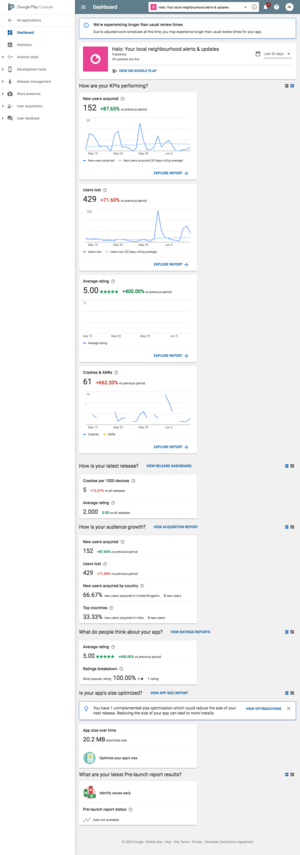
\includegraphics[width=0.4\textwidth]{images/google-play-console/resized-25pct-appdashboardplace_555059634831.png}
  \end{center}
  \caption{Google Play Console Dashboard for LocalHalo Android app}
  \label{fig:gpc-dashboard-for-localhalo-android-resized}
\end{wrapfigure}



\subsubsection{LocalHalo: Findings and Results of the Case Study}
Android Vitals does report a count of crashes, however it does not provide any details of these crashes in Android Vitals, possibly as the overall volumes are low (low tens of crashes per month).


\subsubsection{LocalHalo: Outcomes for the company}


\subsubsection{LocalHalo: Discussion}


\subsubsection{LocalHalo: Contributions to the research and where they are located in the rest of this thesis}

\subsubsection{Earlier stuff follows and needs relocating above here.}



\subsubsection{Experiences of using mobile analytics}
Localhalo incorporate two analytics libraries into their cross-platform mobile application: sentry for crash reporting and mixpanel for business-oriented usage analytics. For their Android app they also have access to Google Play Console.

They experience numerous crashes reported by Sentry, which occur within the React Native runtime environment. Sentry provides email alerts to the development team together with summary reports, (Figure~\ref{fig:localhalo-sentry-weekly-report-21-sep-2020} is example for the period~\nth{14} to~\nth{21} September 2020), and online access to their analytics.

A release in March 2020 had a high crash rate for the production release of their Android app. The top crash cluster was for:

\texttt{java.lang.RuntimeExceptionhost.exp.exponent.experience.a\$b.run}. 

This was traced to a problem in the expo library they used in the app~\url{https://github.com/expo/expo/issues/5839}~\footnote{Expo is a very popular opensource platform for making universal native apps that run on Android, iOS, and the web \url{https://github.com/expo/expo}.}. In that issue several developers for different Android apps provide data from Google Play Console confirming they also receive similar crash clusters. The cause has not yet been definitively traced or addressed, however for the LocalHalo app the crashes stopped being reported once a new release of the Android app, release 1.3.0, was released around \nth{6} April 2020.

In this GitHub issue, 5839, one of the contributors reported their app's crash rate had gone from below 1\% to 10\%~\footnote{\url{https://github.com/expo/expo/issues/5839\#issuecomment-571271045}} and that users were writing terrible reviews. Another contributor observed that the stack trace in Android Vitals is not very useful, what's needed is the error message that appears in the device's log immediately before the stack trace~\footnote{\url{https://github.com/expo/expo/issues/5839\#issuecomment-583838280}}; \phantomsection
\textbf{insight} the stack trace is not always sufficient to understand the failure\label{insight-expo-stack-trace-not-sufficient-to-identify-the-failure}.

\begin{figure}[htbp!]
    \centering
    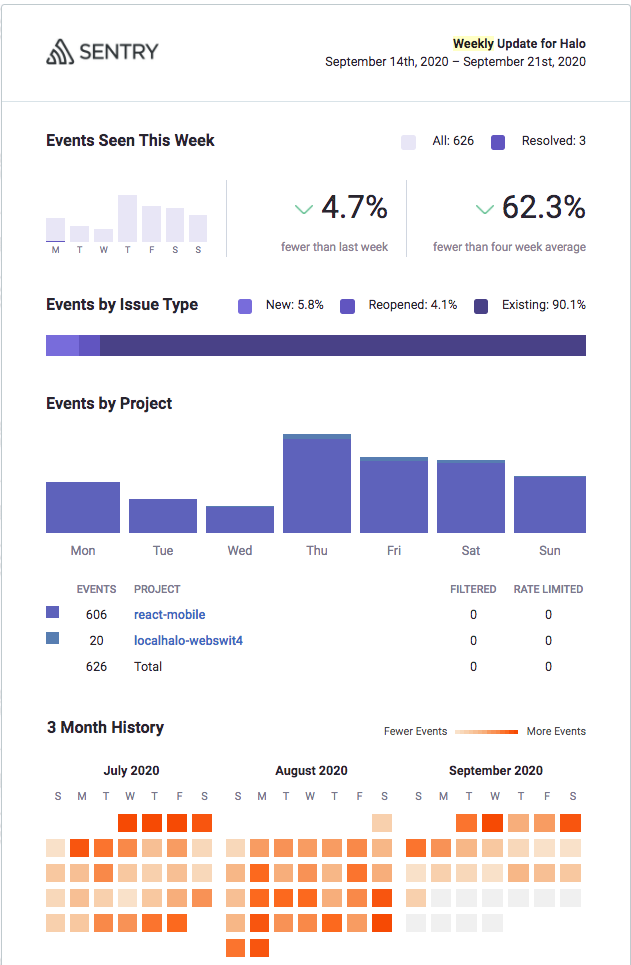
\includegraphics[width=9cm]{images/localhalo/sentry-weekly-report-21-Sep-2020.png}
    \caption{LocalHalo: Sentry weekly report 14 - 21 September 2020}
    \label{fig:localhalo-sentry-weekly-report-21-sep-2020}
\end{figure}

\textbf{Sentry}

MUST-DO Check in Sentry for the various types of error. How actively are the development team reading, reviewing and addressing crashes being reported? 

\begin{figure}[htbp!]
\centering
\begin{minipage}{.5\textwidth}
  \centering
  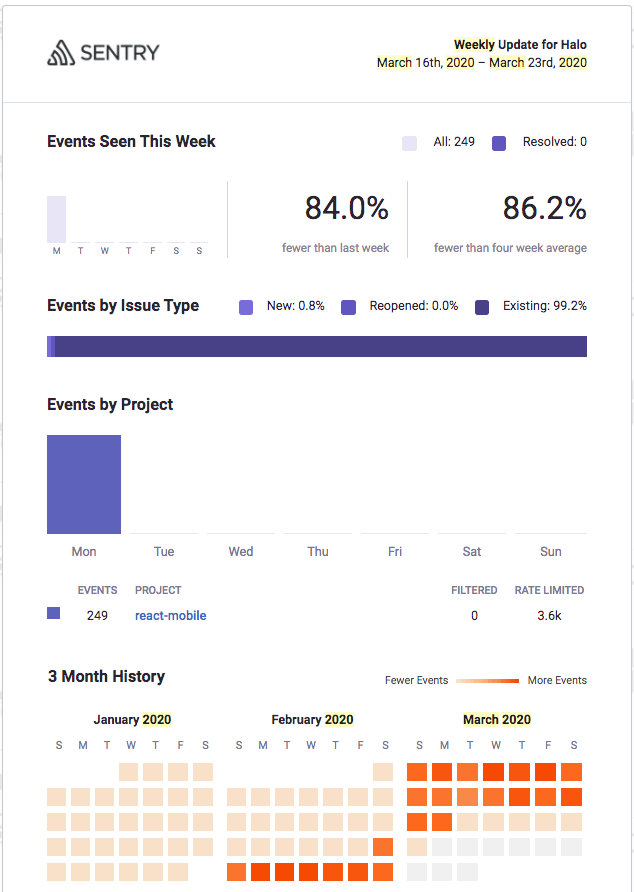
\includegraphics[width=.8\linewidth]{images/localhalo/sentry-weekly-report-16-mar-2020.png}
  \captionof*{figure}{\nth{16} -~\nth{22} March 2020}
  \label{fig:localhalo-sentry-weekly-report-16-mar-2020}
\end{minipage}%
\begin{minipage}{.5\textwidth}
  \centering
  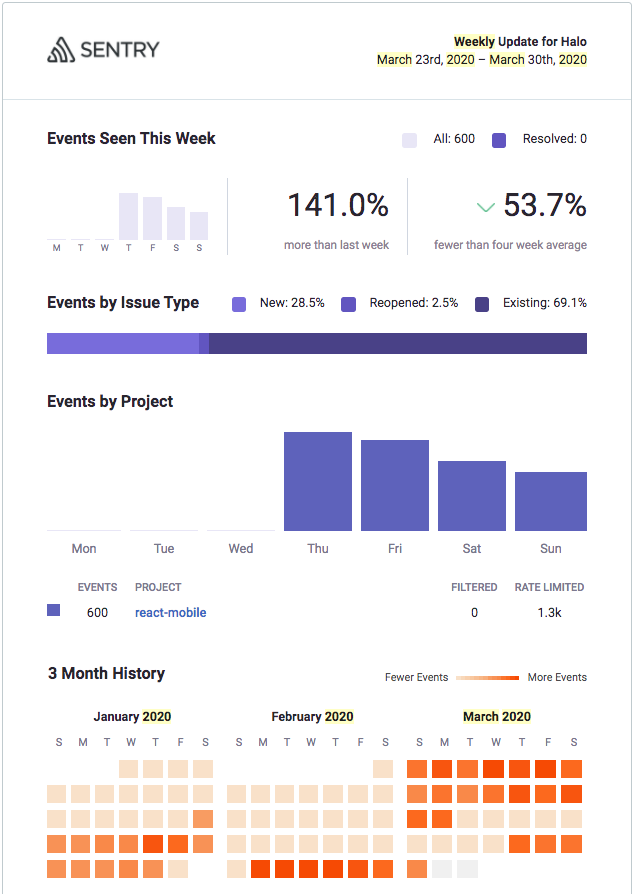
\includegraphics[width=.8\linewidth]{images/localhalo/sentry-weekly-report-23-mar-2020.png}
  \captionof*{figure}{\nth{23} -~\nth{29} March 2020}
  \label{fig:localhalo-sentry-weekly-report-23-mar-2020}
\end{minipage}
    \caption{Missing data reported in Sentry}
    \label{fig:sentry-missing-data-march-2020}
\end{figure}

\begin{comment}


\begin{figure}[htbp!]
    \centering
    %\subfigure[]{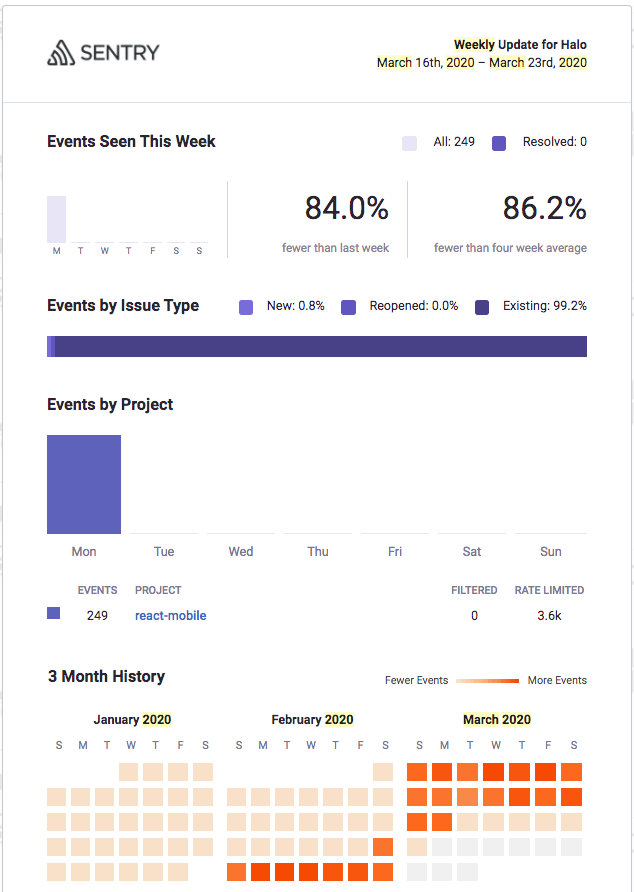
\includegraphics[width=0.4\textwidth]{images/localhalo/sentry-weekly-report-16-mar-2020.png}\caption{\nth{16} -~\nth{22} March 2020}\label{localhalo-sentry-weekly-report-16-mar-2020}}
    \subfigure[]{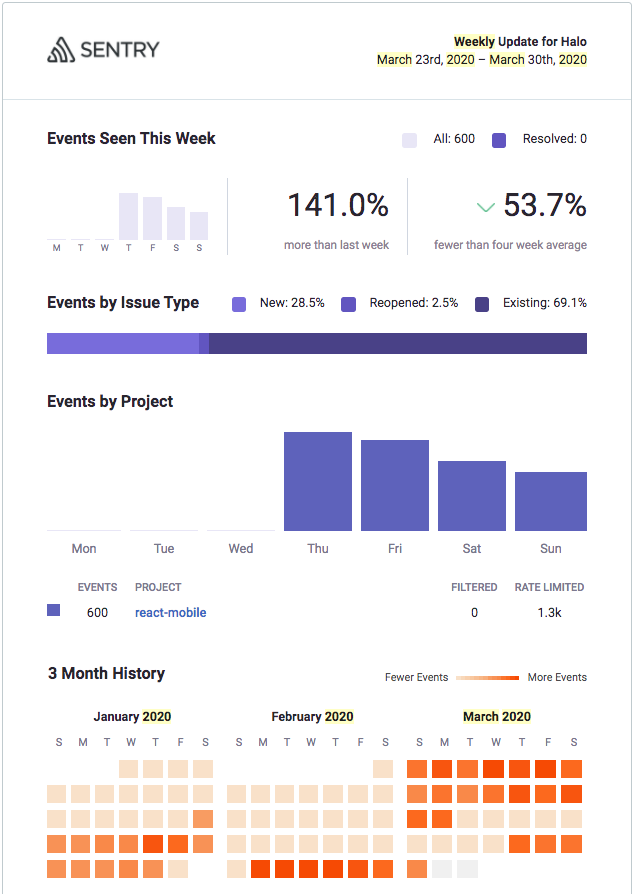
\includegraphics[width=0.4\textwidth]{images/localhalo/sentry-weekly-report-23-mar-2020.png}%\caption{\nth{23} -~\nth{29} March 2020}%\label{localhalo-sentry-weekly-report-23-mar-2020}
    }
    \caption{Missing data reported in Sentry}
    \label{fig:sentry-missing-data-march-2020}
\end{figure}
\end{comment}

%TODO fix the layout of the above figures: try: https://tex.stackexchange.com/questions/37581/latex-figures-side-by-side/37597#37597
Data missing from reports from~\nth{17} March to~\nth{25} March 2020 which affected the statistics around the time of the crashes related to Expo. Figure~\ref{fig:sentry-missing-data-march-2020} illustrates the gap across the two weekly reports. 

SHOULD-DO Consider summarising the crash totals per week. 

\textbf{MUST-DO} write up what we learn from the localhalo case study. external libraries can adversely affect the reliability of apps. Even small development teams can and do use multiple mobile analytics libraries. What can developers learn from the various reports provided by Sentry? How does cross-platform development in react-native affect the app reliability? are there crashes that only occur on Android or iOS? What's the correlation between crashes reported in Android Vitals and Sentry?

Note: The founders of local halo indicated~\footnote{Via their respective LinkedIn profiles: \url{https://www.linkedin.com/in/jamesroutledge/} and \url{https://www.linkedin.com/in/andriymarin/}} they are no longer actively involved in this project, and there are confirming indications in sentry.io as the app has not been updated in over a year, in contrast to the many updates they made previously. So even though the app remains online and available, and the analytics continue to report, there is no one actively maintaining the app or dealing with the errors being reported in the analytics.

\begin{comment}
Extra information available includes:
\begin{itemize}
    \item Their local communities for \href{https://docs.google.com/spreadsheets/d/1iqOvNjRlHIpoRzd61BcBLVkSxGvbta6vrzH2Jgc50aY/htmlview#}{COVID-19 volunteer support communities}.
    \item A social network for neighbors \url{https://ain.ua/en/2019/10/18/localhalo-raises-500k/}
    \item Stack Overflow questions (unpopular and seldom answered) \url{https://stackoverflow.com/questions/tagged/react-native+expo+crash}, a more general search does better \url{https://stackoverflow.com/search?q=\%5Breact-native\%5D+\%5Bexpo\%5D+crash}
    \item Some interesting projects to add device information to react native apps \url{https://github.com/robinpowered/react-native-vitals} and \url{https://github.com/robinpowered/react-native-device-battery}
    \item A long article, with screenshots in Polish or a similar language on publishing react native expo apps to both app stores \url{https://pagepro.co/blog/publishing-expo-react-native-app-to-ios-and-android/}
    \item \href{https://gist.github.com/himgupta229/83b4fd61f294020258976e3edb10b16a}{GitHub GIST: JSON for ANR in Sentry}.
    \item Expo recommends Sentry and documents the integration \url{https://docs.expo.dev/guides/using-sentry/}.
\end{itemize}
\end{comment}